\documentclass[12pt,dvipdfmx]{beamer}
\input{defs}
\title{スケジューリング}
\begin{document}
\maketitle

%%%%%%%%%%%%%%%%%%%%%%%%%%%%%%%%%% 
% \begin{frame}
% \frametitle{目次}
% \tableofcontents
% \end{frame}

%%%%%%%%%%%%%%%%% 
\begin{frame}
  \frametitle{CPUスケジューリング}
  \begin{itemize}
  \item OSの重要な仕事 : スレッドにCPU\footnote{「仮想コア」が正確な言い方だが}を割り当てる
  \item 基本 : かわりばんこ(round robin)
  \item ただし, 文字通り存在するすべてのスレッド
    ($>$ 1,000個は当たり前)に均等時間ずつ, ではない
  \end{itemize}
\end{frame}

%%%%%%%%%%%%%%%%% 
\begin{frame}
  \frametitle{スレッドの状態}
  \begin{itemize}
  \item OSは以下の3つの状態を区別している
    \begin{itemize}
    \item 実行中 (running)
    \item 実行可能 (runnable, active)
    \item 中断中 (blocked, suspended)
    \end{itemize}
  \end{itemize}

  \begin{center}
    \only<1>{\includegraphics[width=\textwidth]{out/pdf/svg/thread_states_1.pdf}}%
    \only<2>{\includegraphics[width=\textwidth]{out/pdf/svg/thread_states_2.pdf}}%
    \only<3>{\includegraphics[width=\textwidth]{out/pdf/svg/thread_states_3.pdf}}%
    \only<4>{\includegraphics[width=\textwidth]{out/pdf/svg/thread_states_4.pdf}}%
  \end{center}
\end{frame}

%%%%%%%%%%%%%%%%% 
\begin{frame}
  \frametitle{スレッドが中断する時の例}
  \begin{itemize}
  \item \ao{OSが, 現在実行中のスレッドがこれ以上実行不能と判断}する時
    \begin{itemize}
    \item \ao{\tt read, recv}などブロッキングI/Oで読むデータがない
    \item \ao{\tt waitpid, pthread\_join}などで, 子プロセス・スレッドが終了していない
    \item \ao{\tt pthread\_mutex\_lock, pthread\_cond\_wait}など同期APIで
      同期が成立していない(次週以降)
    \item \ao{sleep, usleep, nanosleep}など休眠API
    \item ページフォルト(次週以降)でI/Oが発生
    \end{itemize}
  \item OSは, 現在実行中のスレッドから, 別のスレッドに切り替える
    (\ao{コンテクストスイッチ})
  \end{itemize}
  \begin{center}
    \includegraphics[width=0.5\textwidth]{out/pdf/svg/thread_states_2.pdf}
  \end{center}
\end{frame}

%%%%%%%%%%%%%%%%% 
\begin{frame}[fragile]
  \frametitle{ほとんどのスレッドは中断している}
  \begin{itemize}
  \item {\tt ps auxww, top}コマンドの{\tt STAT}欄
    \begin{itemize}
    \item \ao{R} 実行中または実行可
    \item \ao{S} 中断中 (割り込み可能)
    \item \ao{D} 中断中 (割り込み不可能)
    \item その他 \ldots
    \end{itemize}
    
  \item SとDの違いはあまり気にしなくて良い. Dはそれほど見かけない
  \item まめ知識: Unixのload average (負荷平均)
    $=$ RかD状態にあるスレッド数
    $\approx$ R状態にあるスレッド数(の最近何分かの平均)
  \end{itemize}
\end{frame}

%%%%%%%%%%%%%%%%% 
\begin{frame}[fragile]
  \frametitle{スレッドはどこで中断しているかの観察}
  \begin{itemize}
  \item デバッガ (gdb) で実行中のプロセスをデバッグ可能 (attach)
\begin{lstlisting}
$ gdb
(gdb) attach @{\it pid}@
\end{lstlisting} %$
\item 典型
  \begin{itemize}
  \item poll (複数のファイルディスクリプタからの入力待ち)
  \item read
  \end{itemize}
\end{itemize}
\end{frame}

%%%%%%%%%%%%%%%%% 
\begin{frame}
  \frametitle{タスクキュー, ランキュー}
  \begin{itemize}
  \item 実行中・実行可状態のスレッドを維持する
    \begin{itemize}
    \item 「キュー」とは言うがFIFOとは限らない
    \end{itemize}
  \item OSはスレッドを切り替える際,
    ランキュー中から, \ao{ある基準(後述)}に従って次のスレッドを選んで実行する
  \end{itemize}

  \begin{center}
    \includegraphics[width=0.8\textwidth]{out/pdf/svg/run_queue_1.pdf}
  \end{center}
  
\end{frame}

%%%%%%%%%%%%%%%%% 
\begin{frame}
  \frametitle{Preemption (横取り)}
  \begin{itemize}
  \item スレッドが自発的にOSに制御を渡さない
    (なにもシステムコールを呼ばずに走り続けている)状態でも,
    強制的に制御を奪うこと($\equiv$ \ao{preemption})
  \item preemptionを行うスケジューラ $\equiv$ \ao{preemptive}なスケジューラ
  \item 今日のOSのスケジューラは事実上すべてがpreemptive
  \item preemptionを実現する仕組み: \ao{タイマ割り込み}
  \end{itemize}
\end{frame}

%%%%%%%%%%%%%%%%% 
\begin{frame}[fragile]
  \frametitle{割り込み, タイマ割り込み}
  \begin{itemize}
  \item [] 生のCPU (仮想コア): 以下を繰り返す
{\small    
\begin{tabbing}
aa\=aa\=aa\kill                                        
while (1) \{                                           \\
\> PCの指すアドレスから命令を読む                      \\
\> 命令を実行する(一部のレジスタが書き換わる, PC含め)  \\
\> \only<2->{if (割り込みが来た) \{}                              \\
\>\> \only<2->{PC := 割り込みベクタ[割り込み番号];}               \\
\> \only<2->{\}}                                                  \\
\}                                                     \\
\end{tabbing}}
\item[] 注: PC $=$ プログラムカウンタレジスタ
\end{itemize}

\begin{columns}
  \begin{column}{0.8\textwidth}
    \begin{center}
      \only<1>{\includegraphics[width=0.8\textwidth]{out/pdf/svg/interrupt_1.pdf}}%
      \only<2>{\includegraphics[width=0.8\textwidth]{out/pdf/svg/interrupt_2.pdf}}%
      \only<3>{\includegraphics[width=0.8\textwidth]{out/pdf/svg/interrupt_3.pdf}}%
    \end{center}
  \end{column}
  \begin{column}{0.2\textwidth}
    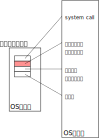
\includegraphics[width=\textwidth]{out/pdf/svg/interrupt_vector.pdf}
  \end{column}
\end{columns}

\end{frame}


%%%%%%%%%%%%%%%%% 
\begin{frame}
  \frametitle{ランキューの動き}
  \only<1>{ランキューには実行可・実行中のスレッドが入っている}%
  \only<2>{実行中のスレッドが中断 $\rightarrow$ ランキューから外れる}%
  \only<3>{ランキューから次のスレッドが選ばれて実行される}%
  \only<4>{中断中のスレッドが再開 $\rightarrow$ ランキューに挿入される}%
  \only<5>{タイマ割り込み $\rightarrow$ 実行中のスレッドが十分な時間を消費していたら, preemption}%
  \only<6>{ランキューから次のスレッドが選ばれて実行される}%

  \begin{center}
    \only<1>{\includegraphics[width=0.8\textwidth]{out/pdf/svg/run_queue_1.pdf}}%
    \only<2>{\includegraphics[width=0.8\textwidth]{out/pdf/svg/run_queue_2.pdf}}%
    \only<3>{\includegraphics[width=0.8\textwidth]{out/pdf/svg/run_queue_3.pdf}}%
    \only<4>{\includegraphics[width=0.8\textwidth]{out/pdf/svg/run_queue_4.pdf}}%
    \only<5>{\includegraphics[width=0.8\textwidth]{out/pdf/svg/run_queue_5.pdf}}%
    \only<6>{\includegraphics[width=0.8\textwidth]{out/pdf/svg/run_queue_6.pdf}}%
  \end{center}
\end{frame}

%%%%%%%%%%%%%%%%% 
\begin{frame}
  \frametitle{スレッド選択}
  \begin{itemize}
  \item OSはスレッドを切り替える際,
    ランキュー中から, \ao{ある基準}に従って次のスレッドを選んで実行する
  \item \ao{ある基準}の例
    \begin{itemize}
    \item Round Robin (純粋なかわりばんこ)
    \item Linux Completely Fair Scheduler (CFS)
    \end{itemize}
  \end{itemize}
\end{frame}

%%%%%%%%%%%%%%%%% 
\begin{frame}
  \frametitle{Round Robin}
  \begin{itemize}
  \item ランキューが純粋なFIFO
  \item 中断から回復したらキューの末尾に入る
  \item 実行中のスレッドのtime quantumがexpireしたら末尾に入る
  \item 次のスレッドを選ぶ際はキューの先頭が選ばれる
  \end{itemize}
\end{frame}

%%%%%%%%%%%%%%%%% 
\begin{frame}
  \frametitle{Round Robinの問題点}
  \begin{itemize}
  \item 公平性: 「中断していた$\iff$CPUを使っていなかった」スレッドも,
    「preemptyされた$\iff$ずっとCPUを使っていた」スレッドも同じ扱い
  \item 対話的なプログラムの応答性: 実行可のスレッドが多い(load averageが高い)と,
    それに比例して,
    「応答時間$=$中断状態から再開してから実行されるまでの時間」が長くなる
  \end{itemize}
\end{frame}

%%%%%%%%%%%%%%%%% 
\begin{frame}
  \frametitle{Linux Completely Fair Scheduler (CFS)}
  \begin{itemize}
  \item Linux 2.6.23以降のデフォルトスケジューラ
    \begin{itemize}
    \item 各スレッドが「消費した合計CPU時間($\rightarrow$ vruntime)」を管理 
    \item スレッド切り替え(実行中スレッドが中断した,
      中断中スレッドが復帰した,
      タイマ割り込みがおきた, など)時に,
      実行可能スレッド中でvruntimeが最小のスレッドを次に実行する
    \item 注: ランキューを,
      vruntimeの小さい順にスレッドが並ぶ優先度キューとすれば実現可能
    \end{itemize}
  \item 効果
    \begin{itemize}
    \item 長い目で見て, 各スレッドへのCPU割当時間を均等にすることができる
      \mbox{$\rightarrow$公平}
    \item しばらく中断していた(CPUを使っていなかった)スレッドが再開した時,
      その間実行されていたスレッドよりもvruntimeが小さいことが期待される
      \mbox{$\rightarrow$対話的スレッドの応答性が高い}
    \end{itemize}
  \end{itemize}
\end{frame}

%%%%%%%%%%%%%%%%% 
\begin{frame}
  \frametitle{vruntime}
  \begin{itemize}
  \item 文字通り, 「vruntime $=$ 割り当てたCPU時間の合計」とするのは問題がある
    \begin{itemize}
    \item 作られたばかりのスレッドのvruntime = 0 $\Rightarrow$ すでにvruntime=10秒
      のスレッドは10秒間待たされる?
    \item 中断していたスレッドのvruntimeは一切増えない
      $\Rightarrow$ 10秒間中断してから再開した時, その10秒間ずっと走っていた
      スレッドは10秒間待たされる?
    \end{itemize}
  \item 「公平にCPUを割当る」と言っても, 「長時間に渡った合計が均等」が目標ではない
    (長時間中断していてもその分を無制限に「貯金」されては困る)
  \end{itemize}
\end{frame}

%%%%%%%%%%%%%%%%% 
\begin{frame}
  \frametitle{vruntime管理の実際}
  \begin{enumerate}
  \item 生成時は親のvruntimeを継承. 親スレッド$A$が子スレッド$B$を生成
    \[ B{\tt .vruntime} = A{\tt .vruntime} \]
  \item タイマ割り込み, スレッド中断時に, 実行中だったスレッド$T$のvruntimeを加算. 
    \[ T{\tt .vruntime \mbox{\tt\ += }} T\mbox{が今回消費したCPU時間} \]
  \item スレッド$T$が中断から復帰する時は,
    $T$のvruntimeが他の実行可・中スレッドよりも極端に小さくならないことを保証
    \[ T{\tt .vruntime} = \max(T{\tt .vruntime}, \min_{t:\mbox{{\scriptsize 実行可}}}t{\tt .vruntime} - 20\mbox{ ms}) \]
  \end{enumerate}
\end{frame}

\end{document}
